\documentclass[12font]{article}
\title{\textbf{Quantum Magic in the Kitaev Model}}
\author{Chen-Chih Wang  }
\date{\textit{Department of Physics, National Tsing Hua University, Hsinchu 30013, Taiwan} \\ (Dated: \today)}
\usepackage[margin=2cm]{geometry}
%\usepackage[fleqn]{amsmath}
%\usepackage{CJK,amsmath}
\usepackage{amsfonts,amssymb}
\usepackage{amsmath}
\numberwithin{equation}{section}    % numbering equations by their section
\usepackage{fancyhdr}
%\pagestyle{fancy}
\usepackage{textcomp}
\usepackage{graphicx}
\usepackage{float}
\usepackage{color}
\usepackage{tikz}
\usepackage{multicol}
\usepackage{threeparttable}
\usepackage{amsthm}
\usepackage{mathtools}
\usepackage{hyperref}
\urlstyle{same}
\usepackage{caption}
\usepackage{subcaption}
\usepackage{dsfont}
\usepackage{qcircuit} % quantum circuit

\usepackage{mathrsfs} % for \mathscr

\usepackage{algorithm}
\usepackage{algpseudocode}

\usepackage{tensor-network}
\tnsetup{tensorsize=16pt, xscale=0.9, yscale=0.6, outer ysep=7pt}

\newtheorem{theorem}{Theorem}[section]
\theoremstyle{definition}
\newtheorem{definition}{Definition}[section]
\newtheorem{lemma}[theorem]{Lemma}
\newtheorem{corollary}{Corollary}[theorem]
\newtheorem{proposition}[theorem]{Proposition}

\hypersetup{
    colorlinks=true,
    linkcolor=blue,
    filecolor=magenta,      
    urlcolor=blue,
    pdftitle={Overleaf Example},
    pdfpagemode=FullScreen,
    }
\usepackage[numbers,sort&compress]{natbib}

\newcommand{\vac}{\mrm{vac}}
\newcommand{\Bra}[1]{\left\langle #1 \right|}
\newcommand{\Ket}[1]{\left| #1 \right\rangle}
\newcommand{\bra}[1]{\langle #1 |}
\newcommand{\ket}[1]{| #1 \rangle}
\newcommand{\anglelr}[1]{\langle #1 \rangle}
\newcommand{\Anglelr}[1]{\left\langle #1 \right\rangle}
\newcommand{\braket}[2]{\langle #1 | #2 \rangle}
\newcommand{\Bbraket}[2]{\left\langle #1 \right|\left. #2 \right\rangle}
\newcommand{\dif}[1]{\frac{\mathrm{d}}{\mathrm{d}#1}}
\newcommand{\diff}[2]{\frac{\mathrm{d}#1}{\mathrm{d}#2}}
\newcommand{\gd}{\boldsymbol{\nabla}}
\newcommand{\dive}{\boldsymbol{\nabla}\cdot}
\newcommand{\curl}{\boldsymbol{\nabla}\times}
\newcommand{\lrno}[1]{\left.#1\right.}
\newcommand{\lr}[1]{\left(  #1  \right)}
\newcommand{\lrm}[1]{\left[  #1  \right]}
\newcommand{\lrg}[1]{\left\{  #1  \right\}}
\newcommand{\lri}[1]{\left. #1 \right.}  % invisible bracket
\newcommand{\abs}[1]{\left|  #1  \right|}
\newcommand{\de}{\partial}
\newcommand{\pdif}[1]{\frac{\partial}{\partial#1}}
\newcommand{\pdiff}[2]{\frac{\partial#1}{\partial#2}}
\newcommand{\mrm}[1]{\mathrm{#1}}
\newcommand{\bo}[1]{\mathbf{#1}}
\newcommand{\bog}[1]{\boldsymbol{#1}}
\newcommand{\vint}[3]{\int_{#1}#2\cdot\mathrm{d}\mathbf{#3}}
\newcommand{\voint}[3]{\oint_{#1}#2\cdot\mathrm{d}\mathbf{#3}}
\newcommand{\Vint}{\int\mrm{d}^3\bo{r}'}
\newcommand{\rr}{\mathbf{r} - \mathbf{r}'}
\newcommand{\arr}{\left|\mathbf{r} - \mathbf{r}'\right|}
\newcommand{\nx}{\hat{\bo{n}}_1}
\newcommand{\ny}{\hat{\bo{n}}_2}
\newcommand{\alert}[1]{{\color{red}#1}}
\newcommand{\alertV}[1]{{\color{violet}#1}}
\newcommand{\Tr}{\mrm{Tr}}
\newcommand{\tTr}{\mrm{tTr}}
\newcommand{\tr}{\mrm{tr}}
\newcommand{\norm}[1]{\left\lVert#1\right\rVert}
\newcommand{\tcor}[2]{\langle -ic_{#1}c_{#2} \rangle_M}

\newcommand{\p}{$+$}
\newcommand{\m}{$-$}
\newcommand{\e}{even}
\newcommand{\od}{odd}

\newcommand{\cnot}{\mrm{CNOT}}

\newcommand{\arrequ}[1]{\begin{aligned}#1\end{aligned}}

\newcommand{\Qcirc}[1]{\begin{minipage}[h]{0.7cm}
	\vspace{0pt}
	\Qcircuit @C=1em @R=.7em {#1}
   \end{minipage}}
\newcommand{\dimer}[2]{\sigma_{#1}^{\alpha_{#1#2}}\sigma_{#2}^{\alpha_{#1#2}}}

\begin{document}
\maketitle
\renewcommand\qedsymbol{$\blacksquare$}



\fontsize{12pt}{16pt}\selectfont

\begin{abstract}
    This note aims to clarify the physical meaning of the roles the matter and gauge sectors play in the quantum magic. We compute the \textit{stabilizer R\'enyi entropy} (SRE) of the Kitaev ground state with and without the magnetic field by exploiting the spin-string structure of the Kitaev model. The result shows that the gauge sector acts as a stabilizer, and the magic resource comes completely from the matter sector.
\end{abstract}

\tableofcontents


\section{Stabilizer R\'enyi Entropy of the Kitaev Ground State}
The \textbf{Kitaev ground state is a stabilizer state} due to the Wilson symmetry, and the \textbf{stabilizer group is constituted by the plaquette operators} $\anglelr{\lrg{W_p}}$. It is also worth mentioning that the stabilizer projector can also be understood as a \textit{condensation operator} proposed in Ref.~\cite{Choi-Sanghavi-Shao-Zheng_2025}. The ground state density matrix reads~\cite{wang2026exactorganizationdensitymatrices}
\[
\ket{\mrm{Gnd}}\bra{\mrm{Gnd}} 
= 
\frac{1}{2^{N-N_p}} 
\lr{\frac{\mathds{1} + \tilde{W}_v}{2}} 
\lr{\frac{\mathds{1} + \tilde{W}_h}{2}}
\prod_{p} \lr{\frac{\mathds{1} + W_p}{2}}
\sum_{[\mathfrak{D}]} \mathfrak{C}_{\mathfrak{D}} \Sigma_{\mathfrak{D}}
\]
With this, the overlap of the ground state with the all-up  ferromagnetic state is
\begin{align*}
\abs{\braket{0}{\mrm{Gnd}}}^2
&=
\frac{1}{2^{N-N_p}} 
\bra{0}
\lr{\frac{\mathds{1} + \tilde{W}_v}{2}} 
\lr{\frac{\mathds{1} + \tilde{W}_h}{2}}
\prod_{p} \lr{\frac{\mathds{1} + W_p}{2}}
\sum_{[\mathfrak{D}]} \mathfrak{C}_{\mathfrak{D}} \Sigma_{\mathfrak{D}}
\ket{0} \\
&=
\frac{1}{2^{N+1}} 
\sum_{[\mathfrak{D}]} 
\sum_{\mathcal{C}}
\lr{
\braket{\mathcal{C}}{\mathfrak{D}}
+
\braket{\mathcal{C}\ominus \mathcal{L}_v}{\mathfrak{D}}
+
\braket{\mathcal{C} \ominus \mathcal{L}_h}{\mathfrak{D}}
+
\braket{\mathcal{C}\ominus \mathcal{L}_v\ominus \mathcal{L}_h}{\mathfrak{D}}
}
\\
&=
\frac{1}{2^{N+1}} 
\sum_{[\mathfrak{D}] \subset [\mathfrak{D}_Z]} 
\sum_{\mathcal{C}}
\lrm{
\varphi(\mathcal{C}, \mathfrak{D})
+
\varphi(\mathcal{C}\ominus \mathcal{L}_v, \mathfrak{D})
+
\varphi(\mathcal{C} \ominus \mathcal{L}_h, \mathfrak{D})
+
\varphi(\mathcal{C}\ominus \mathcal{L}_v\ominus \mathcal{L}_h, \mathfrak{D})
}
\\
&
\alert{\text{only vacuum and $Z$ configurations survive}}
\end{align*}
$\mathcal{C}$ represents contractible loops, including the vacuum $\mathcal{C} = \varnothing$.

The ground state, which is a state in the stabilizer space, is
\begin{equation}\label{eq:gnd-as-stab}
    \ket{\mrm{Gnd}}
    =
    \lr{\frac{\mathds{1} + \tilde{W}_v}{2}} 
    \lr{\frac{\mathds{1} + \tilde{W}_h}{2}}
    \prod_{p} \lr{\frac{\mathds{1} + W_p}{2}}
    \lrm{
        \frac{\abs{\braket{0}{\mrm{Gnd}}}^{-1}}{2^{N-N_p}} 
        \sum_{[\mathfrak{D}]} \mathfrak{C}_{\mathfrak{D}}
        \ket{\mathfrak{D}}
    }
\end{equation}
A $\alpha$-\textit{stabilizer R\'enyi entropy} is defined as~\cite{Leone-Oliviero-Hamma_2022},
\begin{equation}\label{eq:stab-renyi-def}
    M_{\alpha}\lr{\ket{\psi}} := 
    \frac{1}{1 - \alpha} 
    \ln\lr{
        \sum_{\mathsf{S}\in\tilde{\mathcal{P}}_N}
        \frac{1}{2^N}
        \Tr\lr{\rho\mathsf{S}}^{2\alpha}
    }
\end{equation}
where $\rho = \ket{\psi}\bra{\psi}$ is the pure state density matrix of $\ket{\psi}$. We need to bear in mind that the definition above given in Ref.~\cite{Leone-Oliviero-Hamma_2022} applies strictly to pure states. For mixed states, such a definition will not be a valid monotone. 

For the Kitaev model, the stabilizer R\'enyi entropy can be calculated straightforwardly as follows
\begin{equation}\label{eq:genral-SRE}
    M_{\alpha}\lr{\ket{\psi}} 
    = 
    \frac{1}{1 - \alpha} 
    \ln\lr{
        \frac{1}{2^N} \sum_{\mathsf{S}\in\tilde{\mathcal{P}}_N}
        \anglelr{\mathsf{S}}^{2\alpha}
    } 
    =
    \frac{1}{1 - \alpha} 
    \ln\lr{
        \frac{1}{2^{N+1}}
        \sum_{\mathfrak{D}}
        \eta_\mathfrak{D}^\alpha
        \mathfrak{C}_\mathfrak{D}^{2\alpha}
    } 
\end{equation}
In the derivation, we need to be careful that $\Sigma_{\mathfrak{D}_{zz}} \propto \Sigma_{\mathfrak{D}_Z}$. Owing to this, we have to divide the summation by two to avoid overcounting. Here we demonstrate the proof of the property that $\anglelr{\mathsf{S}}^2 = \eta_\mathfrak{D}\mathfrak{C}_\mathfrak{D}^2$ if $\mathsf{S} \propto \Sigma_\mathfrak{D}$, which has been used in the above derivation.  Suppose $\Sigma_\mathfrak{D} = c\mathsf{S}$ with $c$ a specific constant. By definition, the phase $\eta_{\mathfrak{D}}$ is given by $\eta_\mathfrak{D} = \anglelr{\Sigma_\mathfrak{D}^2}$. Substituting the assumption into the definition of $\eta_\mathfrak{D}$ gives
\[
\anglelr{\Sigma_\mathfrak{D}^2} = \eta_\mathfrak{D} = \anglelr{c^2\mathsf{S}^2} = c^2
\]
With this result, we ultimately have the following.
\[
\anglelr{\mathsf{S}}^2 = \frac{1}{c^2}\anglelr{\Sigma_\mathfrak{D}}^2 = \eta_\mathfrak{D}\mathfrak{C}_\mathfrak{D}^2
=
\mrm{Pf}\lr{\mathsf{C}_\mathfrak{D}}^2
\]
For a pure Kitaev model, the phase $\eta_\mathfrak{D} = 1$ is trivial if $[\mathfrak{D}] \in \bo{G}$. Therefore, the ultimate form of the stabilizer R\'enyi entropy of the Kitaev ground state reduces to the following
\begin{equation}
    M_\alpha\lr{\ket{\mrm{Gnd}}} 
    =
    \frac{1}{1 - \alpha}
    \ln\lr{
        \frac{1}{2^{N - N_p}}
        \sum_{[\mathfrak{D}] \in \bo{G}}\mathfrak{C}_\mathfrak{D}^{2\alpha}
    }
\end{equation}
As one would expect, the $\alpha = 1$ stabilizer R\'enyi entropy is an indeterminate form due to the normalization condition Eq.~\eqref{eq:weak-condition}. Therefore, computing the $\alpha=1$ entropy requires taking the limit.
\[
    M_1(\ket{\mrm{Gnd}}) 
    = 
    \lim_{\alpha\to 1} 
    \frac{1}{1 - \alpha}
    \ln\lr{
        \frac{1}{2^{N - N_p}}
        \sum_{[\mathfrak{D}]\in\bo{G}}\mathfrak{C}_\mathfrak{D}^{2\alpha}
    }
    =
    -\frac{1}{2^{N-N_p}}
    \sum_{[\mathfrak{D}]\in\bo{G}} \mathfrak{C}_\mathfrak{D}^2
    \ln \mathfrak{C}_\mathfrak{D}^2
\]
\textbf{In the toric code limit}, all non-zero coefficients $\mathfrak{C}_\mathfrak{D} = 1$ reduce to unity, \textbf{rendering $M_\alpha = 0$}~\footnote{Note that there are $2^{N_d} = 2^{N/2} = 2^{N-N_p}$ configurations $[\mathfrak{D}]$ that give finite correlation functions $\mathfrak{C}_\mathfrak{D}$ in the toric code limit.}. This implies that the quantum state is a perfect stabilizer state. Regarding the equivalence between the string algebra and the Majorana fermion representation of the edge configurations, the above equations imply that the magic is governed entirely by the matter sector. Therefore, it can be sampled using fermionic techniques~\cite{Wang-Yang-Zhou-Chen_2025}.

In general, especially for cases with an external source that breaks TRS, such as a magnetic field, strings with sign factor $\eta_\mathfrak{D} = -1$ can also contribute to the density matrix. Thus, we need to use the most general magic Eq.~\eqref{eq:genral-SRE}. Since both $\eta_\mathfrak{D}$ and $\mathfrak{C}_\mathfrak{D}$ depend only on equivalent classes of the strings, we conclude that
\[
\sum_{\mathfrak{D}} \eta_\mathfrak{D}^\alpha \mathfrak{C}_\mathfrak{D}^{2\alpha}
=
2^{1 + N_p}
\sum_{[\mathfrak{D}]} \eta_\mathfrak{D}^\alpha
\mathfrak{C}_\mathfrak{D}^{2\alpha}
\]
Substituting this into the SRE formula, we obtain
\begin{equation}
    M_\alpha\lr{\ket{\mrm{Gnd}}} 
    =
    \frac{1}{1 - \alpha}
    \ln\lr{
        \frac{1}{2^{N - N_p}}
        \sum_{[\mathfrak{D}] } 
        \eta_\mathfrak{D}^\alpha \mathfrak{C}_\mathfrak{D}^{2\alpha}
    }
\end{equation}

\subsection{Reduced Density Matrix Stabilizer R\'enyi Entropy}
The stabilizer R\'enyi entropy can be extended to general mixed states~\cite{Leone-Oliviero-Hamma_2022}.
\[
\tilde{M}_2\lr{\rho} = 
-\ln\lr{
        \frac{1}{2^N}
        \sum_{\mathsf{S}\in\tilde{\mathcal{P}}_N}
        \Tr\lr{\rho\mathsf{S}}^{4}
    }
- R_2\lr{\rho}
\]
where $R_2\lr{\rho} \equiv -\ln\lr{\Tr\rho^2}$ is the 2-R\'enyi entropy of the state $\rho$.
\begin{equation}\label{eq:red-den-mat-sim-con}
    \rho_A = \frac{1}{2^{N^A-N^A_p}} \mathcal{P}^{(p)}_A\sum_{[\mathfrak{D}]\subset A}\mathfrak{C}_{\mathfrak{D}}\Sigma_{\mathfrak{D}},
\end{equation}
\begin{align*}
    \Tr_A\rho_A^2
    &=
    \frac{1}{2^{2\lr{N^A - N^A_p}}}
        \sum_{[\mathfrak{D}]\subset A}  \sum_{[\mathfrak{D}']\subset A} \mathfrak{C}_{\mathfrak{D}} \mathfrak{C}_{\mathfrak{D}'} 
        \Tr_A\lr{
            \mathcal{P}^{(p)}_A 
            \Sigma_{\mathfrak{D}} \Sigma_{\mathfrak{D}'}
        } \\
    &= 
    \frac{1}{2^{2\lr{N^A - N^A_p}}}
        \sum_{[\mathfrak{D}]\subset A}  \sum_{[\mathfrak{D}']\subset A} 
        \vartheta\lr{\mathfrak{D},\mathfrak{D}'}
        \mathfrak{C}_{\mathfrak{D}} \mathfrak{C}_{\mathfrak{D}'} 
        \Tr_A\lr{
            \mathcal{P}^{(p)}_A 
            \Sigma_{\mathfrak{D}\ominus\mathfrak{D}'}
        } \\
    &=
    \frac{1}{2^{2\lr{N^A - N^A_p}}}
        \sum_{[\mathfrak{D}]\subset A}  \eta_\mathfrak{D}
        \mathfrak{C}_{\mathfrak{D}}^2 
        \Tr_A  \mathcal{P}^{(p)}_A  
    = 
    \frac{1}{2^{N^A - N^A_p}}
        \sum_{[\mathfrak{D}]\subset A}
        \mathfrak{C}_{\mathfrak{D}}^2 
\end{align*}

\[
    \frac{1}{2^{N^A}}
        \sum_{\mathsf{S}\in\tilde{\mathcal{P}}_{N^A}}
        \lrm{\Tr_A\lr{\rho_A\mathsf{S}}}^{4}
    =
    \frac{1}{2^{N^A}}
    \sum_{\mathsf{S}\in\tilde{\mathcal{P}}_{N^A}}
        \anglelr{\mathsf{S}}^{4}
    =
    \frac{1}{2^{N^A}}
    \sum_{\mathfrak{D}\subset A}
        \eta_\mathfrak{D}^2\mathfrak{C}_\mathfrak{D}^{4}
    =
    \frac{1}{2^{N^A-N^A_p}}
    \sum_{[\mathfrak{D}]\subset A} \mathfrak{C}_\mathfrak{D}^{4}
\]

\begin{equation}\label{eq:RDM-SRE}
    \tilde{M}_2\lr{\rho_A} = 
    -\ln\lr{
        \frac{
        \sum_{[\mathfrak{D}]\subset A} \mathfrak{C}_\mathfrak{D}^4 
        }
        {
        \sum_{[\mathfrak{D}]\subset A}\mathfrak{C}_\mathfrak{D}^2
        } 
    }
\end{equation}
This form has already been proposed in Ref.~\cite{Wang-Yang-Zhou-Chen_2025}.

\[
    \sum_{[\mathfrak{D}]\subset A}\mathfrak{C}_\mathfrak{D}^2
    =
    \sum_{\mrm{EP}(\mathfrak{D}) \subset R} \lrm{\mrm{Pf}(\mathsf{C}_\mathfrak{D})}^2 
    =
    \sum_{\mrm{EP}(\mathfrak{D}) \subset R} \det(\mathsf{C}_\mathfrak{D})
    = 
    \det\lr{\mathds{1} + \mathsf{C}_A}
\]

\[
\Gamma_A = \frac{1}{2}\mathds{1} + \frac{i}{2} \mathsf{C}_A
\]
Since the spectrum of the correlation matrix $\Gamma_A$ is the single-particle entanglement spectrum 
\[
\gamma_{k,\pm} = \frac{1 \pm \nu_{k}}{2} \;, \qquad k = 1,2,\cdots, \frac{N^A}{2}
\]
of the reduced density matrix $\rho_A$ of the subregion $A$, the eigenvalues of $\mathsf{C}_A$ are 
\begin{equation}\label{eq:CA-eigen}
    \pm i\frac{\nu_k}{2} \;,\qquad k = 1,2,\cdots, \frac{N^A}{2}.
\end{equation}
Therefore, the 2-R\'enyi entropy reduces to
\begin{align*}
    -\ln\lr{ \frac{1}{2^{N^A-N^A_p}} \sum_{[\mathfrak{D}]\subset A} \mathfrak{C}_\mathfrak{D}^2}
    &=
    -\ln\det\lr{\mathds{1} + \mathsf{C}_A} + \lr{N^A - N^A_p}\ln 2 \\
    &=
    -\ln\lrm{\prod_{k = 1}^{N^A/2} \frac{1}{2}\lr{1 + i\nu_k}\lr{1 - i\nu_k} } + \lr{\frac{N^A}{2} - N^A_p}\ln 2 \\
    &= -\sum_{k=1}^{N^A/2}\ln\lr{\frac{1 + \nu_k^2}{2}} + \lr{\frac{1}{2}\abs{\de A} - 1}\ln 2 
\end{align*}
Now, let's turn to the Pauli spectrum. Since any skew-symmetric matrix can be represented in the standard form, according to Eq.~\eqref{eq:CA-eigen}, there exists an orthogonal $O$ such that 
\[
\mathsf{C}_A = 
O 
\lrm{
    \bigoplus_{k=1}^{N^A/2} \nu_k 
    \begin{pmatrix}
        0 & -1 \\
        1 & 0
    \end{pmatrix}
}
O^T
\]
where $\lrg{\pm \nu_k}$ is the set of eigenvalues of $\mathsf{C}_A$. 

A submatrix $\mathsf{C}_\mathfrak{D}$ having a finite Pffafian $\mathfrak{C}_\mathfrak{D} = \mrm{Pf}(\mathsf{C}_\mathfrak{D})$ 

\[
\det\begin{pmatrix}
    A & B \\
    C & D
\end{pmatrix}
=
\det(A)\det(D - CA^{-1}B)
\]
\[
\det\begin{pmatrix}
    \mathds{1} & \Gamma \\
    -\Gamma^T & \mathds{1}
\end{pmatrix}
=
\det\lr{\mathds{1} + \Gamma^T \Gamma}
\]

% \[
% \mathsf{C}_\mathfrak{D} = 
% O_\mathfrak{D}
% \lrm{
% \bigoplus_{k\in \mathfrak{D}}
% \nu_k
% \begin{pmatrix}
%     0 & -i \\
%     i & 0
% \end{pmatrix}
% }
% O_\mathfrak{D}^T
% \]
% \[
% \mrm{Pf}(\mathsf{C}_\mathfrak{D}) = \prod_{k\in \mrm{sepc}(\mathfrak{D})}\nu_k
% \]
% \[
% \sum_{[\mathfrak{D}]\subset A} \mathfrak{C}_\mathfrak{D}^{2\alpha}
% =
% \sum_{\mrm{spec}(\mathfrak{D}) \subset [N^A]}\prod_{k\in\mrm{spec}(\mathfrak{D})} \nu_k^{2\alpha}
% =
% \lr{1 + \nu_k^{2\alpha}}^{N^A}
% \]

\alert{
\textbf{\underline{Question:}} Does $\tilde{M}(\rho_A) = 0$ implies $M(\ket{\psi}) = 0$? 
}





%%%%%%%%%%%%%%%%%%%%%%%%%%%%%%%
\appendix
%%%%%%%%%%%%%%%%%%%%%%%%%%%%%%%
\section{Minimal Size for Non-trivial Topology}
For numerical efficiency, we tend to choose the smallest possible system. However, the system must still be sufficiently large such that the topological order still exists. A requirement for this is that the ground state manifold should possess four independent topological sectors generated by global Wilson loops if the geometry of the system is a torus.

We start from the Wen plaquette model. There are two requirements for a Wen plaquette system to possess four topologically degenerate ground states:
\begin{itemize}
    \item The lattice must contain an even number of rows or columns in both the horizontal and vertical directions.
    
    \item A global Wilson loop cannot be generated or destroyed by local plaquette operators.
\end{itemize}
The physical meaning of the first requirement is to preserve the checkerboard pattern of the lattice. If there are adjacent plaquettes (cells) that are of the same type (black or white, in a checkerboard sense), then the two types of plaquettes become identical, and the original two different Wilson loops become the same. This breakdown of the checkerboard pattern reduces the original fourfold topological ground state degeneracy down to twofold, which is not adequate to describe the physics of a toric code system.

According to the two requirements, \textbf{the smallest possible topologically non-trivial Wen plaquette model contains eight ($8 = 2\times 4$) distinct plaquettes and eight sites}. A $2\times 2$ checkerboard is not adequate for the system to have four topological sectors since it violates the second requirement\footnote{The \textit{global Wilson loop} is identical to a plaquette operator}. 

\begin{figure}
    \centering
    (a)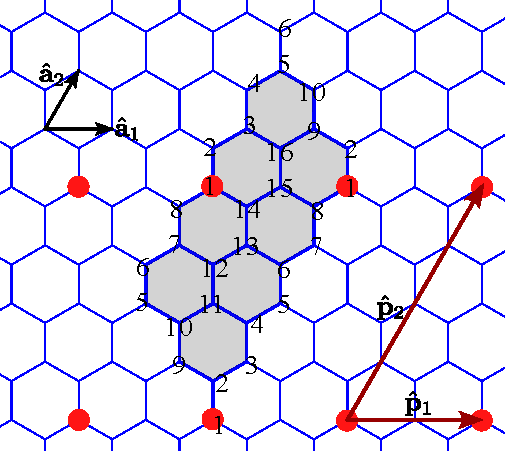
\includegraphics[height=0.15\textheight]{figures/minimal-system.pdf}
    \hspace{5mm}
    (b)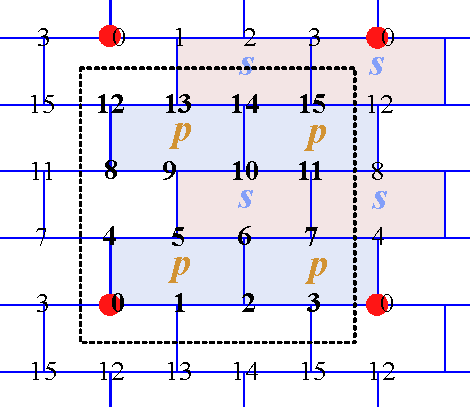
\includegraphics[height=0.15\textheight]{figures/minimal-system_brick-wall.pdf}
    \hspace{5mm}
    (c)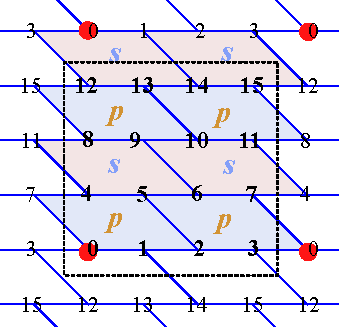
\includegraphics[height=0.15\textheight]{figures/minimal-system_brick-wall_diagonal.pdf}
    \caption{(a) The smallest topologically non-trivial system consists of 8 unit cells, which is equivalent to 16 spins. The two vectors that define the periodic boundary condition are $\hat{\bo{p}}_1 = 2\hat{\bo{a}}_1$ and $\hat{\bo{p}}_2 = 4\hat{\bo{a}}_2$, respectively. (b) For numerical simplicity, the honeycomb lattice is rearranged into a brick-wall geometry, and the spins are relabeled according to their Euclidean coordinates in the lattice. In both figures, red dots indicate identical lattice sites. (c) An equivalent choice.}
    \label{fig:lattice}
\end{figure}

\section{Finite-Size Correlation}
As mentioned in our work~\cite{wang2026exactorganizationdensitymatrices}, at the ground state, the multi-spin correlation function of the Kitaev model is finite if and only if it can be written in the form of a string. Therefore, we only need to discuss the following form of the correlation function
\[
\Anglelr{
    \prod_{\anglelr{ij}\in\mathfrak{D}}
    \dimer{i}{j}
}
\]
This kind of correlation function can be exactly evaluated in the Majorana representation. Substituting the transformation 
\[
\dimer{i}{j} \to i b^{\alpha_{ij}}_i c_i  i b^{\alpha_{ij}}_j c_j = \hat{u}_{ij} ic_jc_i
\]
into the correlation function and taking the trivial gauge, we have
\[
\Anglelr{
    \prod_{\anglelr{ij}\in\mathfrak{D}}
    \dimer{i}{j}
}
=
\Anglelr{
    \prod_{\anglelr{ij}\in\mathfrak{D}}
    (-i) c_ic_j
}_M
\]
Therefore, we only need to focus on the two-point correlation functions. Here we set the system to satisfy the \textbf{periodic boundary condition}, which is characterized by two independent vectors, $\hat{\bo{p}}_1 = 2\hat{\bo{a}}_1$ and $\hat{\bo{p}}_2 = 4\hat{\bo{a}}_2$, as illustrated in Fig.\ref{fig:lattice}.a. The geometry adopted here follows the one illustrated in Ref.~\cite{Pedrocchi-Chesi-Loss_2011}

\subsection{Momentum States in Finite Systems}
For slave fermions in the parton construction, the system boundary condition can be periodic (PBC) or anti-periodic (APBC), depending on the chosen topological sector~\cite {Kou-Levin-Wen_2008}. Here, we only consider the PBC in both horizontal and vertical directions. 
\begin{equation}\label{eq:PBC}
    f_{\sigma\mu\bo{x}} = f_{\sigma\mu,(\bo{x} + \hat{\bo{p}}_1)} = f_{\sigma\mu,(\bo{x} + \hat{\bo{p}}_2)}
\end{equation}
To determine the allowed momentum states, we first Fourier transform the fermions as follows
\[
f_{\sigma\mu\bo{x}} = \frac{1}{\sqrt{N/2}}\sum_{\bo{k}} e^{i\bo{k}\cdot\bo{x}} f_{\sigma\mu\bo{k}}
\]
With this expression, Eq.~\eqref{eq:PBC} implies that the allowed momentum $\bo{k}$ must satisfy
\begin{equation}\label{eq:condition-init}
    \left\{
    \begin{array}{lll}
        \bo{k}\cdot\hat{\bo{p}}_1 = 2n_1\pi & ; & n_1 = 0,1,\cdots,N_h-1\\
        \bo{k}\cdot\hat{\bo{p}}_2 = 2n_2\pi & ; & n_2 = 0,1,\cdots,N_v-1
    \end{array}
    \right.
\end{equation}
In our case illustrated in Fig.~\ref{fig:lattice}, $N_h=2$ and $N_v = 4$, representing the number of unit cells included in the system in the horizontal and vertical directions, respectively. Consider the unit vectors $\hat{\bo{a}}_1 = \hat{\bo{e}}_x$ and $\hat{\bo{a}}_2 = \frac{1}{2}\hat{\bo{e}}_x + \frac{\sqrt{3}}{2}\hat{\bo{e}}_y$. We can define the unit vectors in the momentum space as 
\[
\left\{
\begin{aligned}
& \hat{\bo{b}}_1 =  2\pi\hat{\bo{e}}_x - \frac{2\pi}{\sqrt{3}}\hat{\bo{e}}_y\\
& \hat{\bo{b}}_2 = \frac{4\pi}{\sqrt{3}}\hat{\bo{e}}_y
\end{aligned}
\right.
\]
such that $\hat{\bo{a}}_i\cdot\hat{\bo{b}}_j = 2\pi \delta_{ij}$. With these basis vectors, the allowed momentum states are
\begin{equation}\label{eq:allowed-momentum}
    \bo{k} = \frac{n_1}{2}\hat{\bo{b}}_1 + \frac{n_2}{4}\hat{\bo{b}}_2 \quad ; \quad n_1=0,1 \quad,\quad n_2=0,1,2,3
\end{equation}

In general, if the relation between two representations $\bo{k} = k_x\hat{\bo{e}}_x + k_y\hat{\bo{e}}_y = k_1\hat{\bo{b}}_1 + k_2\hat{\bo{b}}_2$ is
\[
\begin{array}{ccc}
    \left\{
    \begin{aligned}
        & k_x = 2\pi k_1 \\
        & k_y = \frac{2\pi}{\sqrt{3}}\lr{-k_1 + 2k_2}
    \end{aligned}
    \right.
    &  
    ,
    &
    \left\{
    \begin{aligned}
        & k_1 = \frac{1}{2\pi} k_x \\
        & k_2 = \frac{1}{4\pi}\lr{k_x + \sqrt{3}k_y}
    \end{aligned}
    \right.
\end{array}
\]


\subsection{Two-Points Correlation Functions}
The correlation functions can be calculated more easily in the normal fermion language. As defined in the appendix, the $c$-Majorana fermions can be written in terms of $\gamma$-fermions,
\[
\left\{
\begin{aligned}
& c_{\bo{x}A} =  \gamma^\dagger_{\bo{x}} + \gamma_{\bo{x}} = \frac{1}{\sqrt{N/2}}\sum_{\bo{k}}\lr{\gamma^\dagger_k e^{-ik\bo{x}} + \gamma_{\bo{k}} e^{ik\bo{x}}} \\
& c_{\bo{x}B} = i\lr{\gamma^\dagger_{\bo{x}} - \gamma_{\bo{x}}} = \frac{i}{\sqrt{N/2}}\sum_{\bo{k}}\lr{\gamma^\dagger_k e^{-ik\bo{x}} - \gamma_{\bo{k}} e^{ik\bo{x}}}
\end{aligned}
\right.
\]
And the ground state is 
\[
\ket{\psi} = A\exp\lr{\sum_{k\in\mrm{HBZ}}g_k\gamma^\dagger_k\gamma^\dagger_{-k}} \ket{0}
\]
where 
\[
A = \prod_{k\in\mrm{HBZ}}\lr{1 + \abs{g_k}^2}^{-1/2}
\]
is the normalization constant. Similar to Numbu-Gor'kov Green's function, there are two types of fermion pairing, $AA(BB)$ and $AB$. Both types of correlation functions can be simplified to the problem of solving the $\gamma$-fermion correlation function as we will see later. The two $\gamma$-fermion correlation functions we have to know are $\anglelr{\gamma_{\bo{k}}\gamma_{k'}}$ and $\anglelr{\gamma^\dagger_k\gamma_{k'}}$. Their analytical forms are given as follows
\[
\left\{
\begin{aligned}
& \anglelr{\gamma^\dagger_k \gamma_{k'}} = \frac{\abs{g_k}^2}{1+\abs{g_k}^2}\delta_{kk'} = v_k^2\delta_{kk'} = \frac{1}{2}\lr{1-\frac{R_{\bo{k}}}{\abs{s_{\bo{k}}}}}\delta_{kk'}\\
& \anglelr{\gamma_{\bo{k}}\gamma_{k'}} = \frac{g_k}{1+\abs{g_k}^2}\delta_{k,-k'} = i\mrm{sgn}\lr{I_k}u_kv_k\delta_{k,-k'} = i\frac{I_k}{2\abs{s_{\bo{k}}}}\delta_{k,-k'}
\end{aligned}
\right.
\]
and the fermionic commutation relations can give other two types of correlation functions
\[
\left\{
\begin{aligned}
& \anglelr{\gamma_{\bo{k}}\gamma_{k'}^\dagger} = \delta_{kk'} - \anglelr{\gamma^\dagger_{k'}\gamma_{\bo{k}}} = u^2_k\delta_{kk'} = \frac{1}{2}\lr{1+\frac{R_{\bo{k}}}{\abs{s_{\bo{k}}}}}\delta_{kk'} \\
& \anglelr{\gamma_{\bo{k}}^\dagger\gamma_{k'}^\dagger} = \anglelr{\gamma_{k'}\gamma_{\bo{k}}}^* = -i\mrm{sgn}(I_{\bo{k}'})u_{\bo{k}'}v_{\bo{k}'}\delta_{\bo{k}',-\bo{k}} = i\mrm{sgn}(I_{k})u_{\bo{k}}v_{\bo{k}}\delta_{\bo{k},-\bo{k}'} = \anglelr{\gamma_{\bo{k}}\gamma_{\bo{k}'}} \delta_{\bo{k},-\bo{k}'}
\end{aligned}
\right.
\]

Here I list the explicit expressions for $s_k$, $R_k$, and $I_k$, and other relevant quantities or functions. We start from 
\[
s_k = 2\lr{J_x e^{ik\cdot \hat{\bo{n}}_1} + J_y e^{ik\cdot \hat{\bo{n}}_2} + J_z}
\]
Then, if we express the momentum state in terms of $\bo{k} = k_x\hat{\bo{e}}_x + k_y\hat{\bo{e}}_2$, then
\begin{equation}\label{eq:functions}
  \left.
  \begin{aligned}
  &\abs{s_k} = 2\lrm{J_x^2+J_y^2+J_z^2 + 2J_xJ_y\cos\lr{k_x} + 2J_xJ_z\cos\lr{\frac{1}{2}k_x+\frac{\sqrt{3}}{2}k_y} + 2J_yJ_z\cos\lr{\frac{1}{2}k_x-\frac{\sqrt{3}}{2}k_y}}^{1/2} \\
  & R_k = 2\lrm{J_x\cos\lr{\frac{1}{2}k_x+\frac{\sqrt{3}}{2}k_y} + J_y\cos\lr{\frac{1}{2}k_x-\frac{\sqrt{3}}{2}k_y} + J_z}\\
  &I_k = 2\lrm{J_x\sin\lr{\frac{1}{2}k_x+\frac{\sqrt{3}}{2}k_y} - J_y\sin\lr{\frac{1}{2}k_x-\frac{\sqrt{3}}{2}k_y}}
  \end{aligned}
  \right\}
\end{equation}
Or, expressed in terms of reciprocal basis vectors $\bo{k} = k_1\hat{\bo{b}}_1 + k_2\hat{\bo{b}}_2$, then
\begin{equation}\label{eq:functions_b}
  \left.
  \begin{aligned}
  &\abs{s_k} 
  = 
  2\lrm{
      J_x^2+J_y^2+J_z^2 + 2J_xJ_y\cos\lr{2\pi k_1} 
      + 
      2J_xJ_z\cos\lr{2\pi k_2} 
      + 
      2J_yJ_z\cos\lr{2\pi (k_1 - k_2)}
  }^{1/2} \\
  & R_k 
  = 2\lrm{
      J_x\cos\lr{2\pi k_2} 
      + 
      J_y\cos\lr{2\pi (k_1 - k_2)} 
      + 
      J_z
  }\\
  &I_k 
  = 2\lrm{
      J_x\sin\lr{2\pi k_2} 
      - 
      J_y\sin\lr{2\pi (k_1 - k_2)}
  }
  \end{aligned}
  \right\}
\end{equation}
Again, these results are general and are valid even in a finite-size system.

With these relations, we can start to compute the $c$-Majorana correlation functions. For $AA$-pairings, the correlation function is,
\begin{align*}
  \anglelr{c_{\bo{x}A}c_{\bo{x}'A}} &= \frac{1}{N/2}\sum_{\bo{k}}\lr{ \anglelr{\gamma_{\bo{k}}\gamma_{-\bo{k}}} + \anglelr{\gamma_{-\bo{k}}^\dagger\gamma^\dagger_{k}} +
  \anglelr{\gamma_{\bo{k}}\gamma_{k}^\dagger} + 
  \anglelr{\gamma_{-\bo{k}}^\dagger\gamma_{-\bo{k}}}
  }e^{i\bo{k}\cdot\lr{\bo{x}-\bo{x'}}} \\
  &= \frac{1}{N/2}\sum_{\bo{k}} e^{i\bo{k}\cdot\lr{\bo{x}'-\bo{x}}} = \delta_{\bo{x}\bo{x}'}
\end{align*}

For $AB$-pairings, a similar calculation gives
\begin{align*}
  \anglelr{c_{\bo{x}A}c_{\bo{x}'B}} &= \frac{i}{N/2}\sum_{\bo{k}}\lr{ \anglelr{-\gamma_{\bo{k}}\gamma_{-\bo{k}}} + \anglelr{\gamma_{-\bo{k}}^\dagger\gamma^\dagger_{k}} +
  \anglelr{\gamma_{\bo{k}}\gamma_{k}^\dagger} - 
  \anglelr{\gamma_{-\bo{k}}^\dagger\gamma_{-\bo{k}}}
  }e^{i\bo{k}\cdot\lr{\bo{x}-\bo{x'}}} \\
  &= \frac{i}{N/2}\sum_{\bo{k}}\lr{\frac{R_{\bo{k}}}{\abs{s_{\bo{k}}}} - i\frac{I_k}{\abs{s_{\bo{k}}}}}e^{i\bo{k}\cdot\lr{\bo{x}'-\bo{x}}} 
  = \frac{i}{N/2}\sum_{\bo{k}}\frac{s^*_{\bo{k}}}{\abs{s_{\bo{k}}}}e^{i\bo{k}\cdot\lr{\bo{x}'-\bo{x}}} 
\end{align*}
This result is purely imaginary and can be further simplified,
\begin{align}\label{eq:correlationAB}
  \anglelr{-ic_{\bo{x}A}c_{\bo{x}'B}} 
  &= 
  \frac{1}{N/2}\sum_{\bo{k}}\cos\lrm{\bo{k}\cdot\lr{\bo{x}'-\bo{x}} - \theta_{\bo{k}}} \nonumber \\
  &= 
  \frac{1}{N/2}
  \sum_{\bo{k}}
  \frac{1}{\abs{s_{\bo{k}}}}\lrm{R_{\bo{k}} \cos\lr{\bo{k} \cdot \delta\bo{x}} + I_{\bo{k}}\sin\lr{\bo{k}\cdot\delta\bo{x}} }
\end{align}
where $s_{\bo{k}} = \abs{s_{\bo{k}}}e^{i\theta_{\bo{k}}}$. Notice that the above formulation is general and can be used directly in the case of finite systems.

\subsection{Two-Points Correlation Functions with an External Magnetic Field}
In the isotropic limit, applying an external magnetic field makes the Kitaev model equivalent to a Haldane honeycomb model~\cite{Haldane_1988} in the Majorana fermion representation. In general, the correlation functions of $AA$ and $BB$ pairings are finite. However, since the $\mathbb{Z}_2$ gauge fields are still c-numbers, the ground state still exhibits the pattern that only string-like operators bear finite expectation values. The only difference is that, in the situation with a magnetic field, the N.N.N. coupling contributes to the correlation functions of longer strings, and strings with both endpoints of the same type have finite expectation values in general. 

If a magnetic field is applied to the system, then the elementary excitations are given in Eq.~\eqref{eq:magnetic-field-elementary-excitation}, which satisfy 
\[
\left\{
\begin{aligned}
    & \anglelr{a^{\dagger}_{\bo{k}} a_{\bo{k}'}} 
    \delta_{\bo{k}\bo{k}'} \\
    & \anglelr{a_{\bo{k}} a_{\bo{k}'}} = \anglelr{a_{\bo{k}} a^{\dagger}_{\bo{k}'}} = 0
\end{aligned}
\right.
\]
Therefore, the $\gamma$-fermions can be represented in terms of the elementary excitations as follows,
\[
\begin{pmatrix}
    \gamma_{\bo{k}} \\
    \gamma^\dagger_{-\bo{k}} 
\end{pmatrix} 
=
\begin{pmatrix}
    u_{\bo{k}} a_{\bo{k}} + e^{-i\varphi_{\bo{k}}} v_k a_{-\bo{k}}^\dagger \\
    e^{i\varphi_{\bo{k}}} v_k a_{\bo{k}} + u_{\bo{k}} a_{-\bo{k}}^\dagger
\end{pmatrix}.
\]

\[
\left\{
\begin{aligned}
    & \anglelr{\gamma_{\bo{k}}^\dagger \gamma_{\bo{k}'}}
    =
    u_{\bo{k}}^2 \delta_{\bo{k}\bo{k}'} 
    =
    \frac{1}{2}\lr{1 + \frac{R_{\bo{k}}}{\epsilon(\bo{k})} } \delta_{\bo{k}\bo{k}'} 
    \\
    & \anglelr{\gamma_{\bo{k}} \gamma_{\bo{k}'}^\dagger} 
    = 
    \frac{1}{2}\lr{1 - \frac{R_{\bo{k}}}{\epsilon(\bo{k})} } \delta_{\bo{k}\bo{k}'} \\
    & \anglelr{\gamma_{\bo{k}} \gamma_{\bo{k}'}} = e^{-i\varphi_{\bo{k}}} v_{\bo{k}} u_{-\bo{k}} \delta_{\bo{k},-\bo{k}'}
    =
    \frac{\Delta_{\bo{k}} - iI_{\bo{k}} }{2\epsilon(\bo{k})} \delta_{\bo{k},-\bo{k}'} \\
    & \anglelr{\gamma^\dagger_{\bo{k}} \gamma^\dagger_{\bo{k}'}} = \anglelr{\gamma_{\bo{k}'} \gamma_{\bo{k}}}^* = 
    -\frac{\Delta_{\bo{k}} + iI_{\bo{k}} }{2\epsilon(\bo{k})} \delta_{\bo{k},-\bo{k}'}
\end{aligned}
\right.
\]
Note that $u_{-\bo{k}} = u_{\bo{k}}$.

There are two types of two-point correlation functions. The first one is the pairing in the same sublattice.
\begin{align*}
  \anglelr{-ic_{\bo{x}A}c_{\bo{x}'A}} 
  &= 
  \frac{-i}{N/2}
  \sum_{\bo{k}}\lr{ \anglelr{\gamma_{\bo{k}}\gamma_{-\bo{k}}} + \anglelr{\gamma_{-\bo{k}}^\dagger\gamma^\dagger_{k}} +
  \anglelr{\gamma_{\bo{k}}\gamma_{\bo{k}}^\dagger} + 
  \anglelr{\gamma_{-\bo{k}}^\dagger\gamma_{-\bo{k}}}
  } e^{i\bo{k}\cdot\lr{\bo{x}-\bo{x'}}} \\
  &= 
  \frac{-i}{N/2}
  \sum_{\bo{k}}
  \lr{
    1 + \frac{\Delta_{\bo{k}}}{\epsilon(\bo{k})}
  } e^{i\bo{k}\cdot\lr{\bo{x}-\bo{x'}}}
\end{align*}

\begin{equation}\label{eq:AA-correlation-magnetic}
   \anglelr{-ic_{\bo{x}A}c_{\bo{x}'A}} 
   =
   -i\delta_{\bo{x}\bo{x}'}
   +
   \frac{1}{N/2}
  \sum_{\bo{k}}
  \frac{\Delta_{\bo{k}}}{\epsilon(\bo{k})}
  \sin\lr{\bo{k}\cdot\delta\bo{x}}
\end{equation}

\begin{align*}
  \anglelr{-ic_{\bo{x}A}c_{\bo{x}'B}} 
  &= 
  \frac{1}{N/2}\sum_{\bo{k}}\lr{ -\anglelr{\gamma_{\bo{k}}\gamma_{-\bo{k}}} + \anglelr{\gamma_{-\bo{k}}^\dagger\gamma^\dagger_{k}} +
  \anglelr{\gamma_{\bo{k}}\gamma_{k}^\dagger} - 
  \anglelr{\gamma_{-\bo{k}}^\dagger\gamma_{-\bo{k}}}
  }e^{i\bo{k}\cdot\lr{\bo{x}-\bo{x'}}} \\
  &= 
  \frac{1}{N/2} \sum_{\bo{k}}
  \lr{
      \frac{R_{\bo{k}}}{\epsilon(\bo{k})} + i\frac{I_k}{\epsilon(\bo{k})}
  } e^{i\bo{k}\cdot\lr{\bo{x}'-\bo{x}}} \\
  &=
  \frac{1}{N/2} \sum_{\bo{k}}
  \frac{\abs{s_k}}{\epsilon(\bo{k})}
  e^{i\bo{k}\cdot\lr{\bo{x}'-\bo{x}} + i\theta_{\bo{k}} } \in \mathbb{R}
\end{align*}

\begin{equation}\label{eq:AB-correlation-magnetic}
    \anglelr{-ic_{\bo{x}A}c_{\bo{x}'B}} 
    =
    \frac{1}{N/2}
    \sum_{\bo{k}}
    \lrm{
        \frac{R_{\bo{k}}}{\epsilon(\bo{k})} \cos\lr{\bo{k}\cdot\delta\bo{x}}
        -
        \frac{I_{\bo{k}}}{\epsilon(\bo{k})} \sin\lr{\bo{k}\cdot\delta\bo{x}}
    }
\end{equation}

\subsection{Nearest Neighbor Correlation Functions}
In the toric code limit, the dominant correlation functions are those of nearest-neighbor lattice sites along the strong coupling direction. Without loss of generality, assume the dominant coupling is $J_z$, so that $J_x$ and $J_y$ can be treated as perturbations. In this case, the term $\abs{s_k}$ appearing in the denominator in the integrand is
\begin{align*}
    \abs{s_k}^{-1}
    &=
    \lrm{
        1 + \delta^2 + \delta^2 + 2\delta\delta \cos\lr{\bo{k}\cdot\lr{\hat{\bo{n}} + \hat{\bo{n}}_2}} + 2\delta \cos\lr{\bo{k}\cdot\hat{\bo{n}}_1} + 2\delta \cos\lr{\bo{k}\cdot\hat{\bo{n}}_2}  
    }^{-1/2} \\
    &\approx
    1 - 
    \frac{1}{2}
    \lrm{
        1 + 2\delta^2 + 2\delta^2 \cos\lr{\bo{k}\cdot\lr{\hat{\bo{n}} + \hat{\bo{n}}_2}} + 2\delta \cos\lr{\bo{k}\cdot\hat{\bo{n}}_1} + 2\delta \cos\lr{\bo{k}\cdot\hat{\bo{n}}_2}
    } \\
    & \qquad
        + 
\end{align*}

\[
\delta
=
\frac{\alpha/3}{1 - 2\alpha/3}
\approx
\frac{\alpha}{3}
+
\frac{2\alpha^2}{9}
\]

\subsection{Two-Points Correlation Functions in a Finite-Size System}
In the following discussions, we consider the lattice geometry illustrated in Fig.~\ref{fig:lattice}.c. In this situation, there are three methods for labeling the position of lattice sites. 
\begin{itemize}
    \item The first method is to assign a number to each lattice site one by one. The label is denoted by $n$ in this note.
    
    \item In the lattice geometry illustrated in Fig.~\ref{fig:lattice}.c, the lattice sites can be sorted into layers labeled by $l$, and the horizontal position of a lattice site in each layer is labeled by $s$, standing for \textit{site}. For example, the position of site number 7 is $(l,s) = (1,3)$, and the position of site number 12 is $(l,s) = (3,0)$. The integer $s$ can be further decomposed as
    \[
    s = 2 s_q + s_r
    \]
    where $s_q \in \mathbb{N}$ and $s_r = 0\vee 1$ is the remainder.

    \item With the Bravais lattice site expressed as $\bo{x} = x\hat{\bo{a}}_1 + y\hat{\bo{a}}_2$, each lattice site corresponds to a unique pair $(\bo{x},\mu)$, where $\mu = 0,1$, with $0$ representing sublattice $B$ and $1$ representing $A$, respectively.

    \item The following equations describe the relationships among the three labeling methods listed above.
    \[
    \left\{
    \begin{aligned}
        & n = s + lN_h \\
        & \mu = n \mod{2}\\
        & x = s_q + s_r \\
        & y = l - s_r
    \end{aligned}
    \right.
    \]
\end{itemize}
With this definition, the factor $\bo{k}\cdot\delta\bo{x}$ in Eq.~\eqref{eq:correlationAB} can be written as
\[
\bo{k}\cdot\delta\bo{x} = \pi \lr{n_1\delta x + \frac{n_4}{2}\delta y}
\]
where $n_1$ and $n_2$ are defined by the expression Eq.~\eqref{eq:allowed-momentum} of momentum states, and $\delta x$ and $\delta y$ are components of the position $\bo{x}$ represented in terms of lattice unit vectors $\bo{x} = \delta x \hat{\bo{a}}_1 + \delta y\hat{\bo{a}}_2$. Using this representation, the summation $\sum_{\bo{k}}$ in Eq.~\eqref{eq:correlationAB} can be written as $\sum_{n_1,n_2}$. The only difference is that the momentum is now represented in terms of integers $n_1$ and $n_2$.

\subsection{String Correlation Functions}
\[
\prod_{\anglelr{ij}\in\mathfrak{D}}
    \dimer{i}{j}
=
\prod_{\mathcal{C} \in \mrm{St}(\mathfrak{D})}
\lr{
    \prod_{\anglelr{ij}\in\mathcal{C}}
    \dimer{i}{j}
}
\]
We have required $\mathcal{C} \in \bo{G}$. That is to say, each string $\mathcal{C}$ connects a type-$A$ and a type-$B$ endpoint.
\begin{align*}
    \prod_{\anglelr{ij}\in\mathcal{C}}
    \dimer{i}{j}
    \to
    \prod_{\anglelr{ij}\in\mathcal{C}}
        (-i) c_ic_j 
    &=
    (-i)^{\abs{\mathcal{C}}} (-1)^{(\abs{\mathcal{C}} - 1)/2}c_{a_{\mathcal{C}}}c_{b_{\mathcal{C}}} \\
    &=
    -i
    (-1)^{\abs{\mathcal{C}}(\abs{\mathcal{C}}+1)/2} (-1)^{(\abs{\mathcal{C}} + 1)/2}c_{a_{\mathcal{C}}}c_{b_{\mathcal{C}}} \\
    &= -i (-1)^{(\abs{\mathcal{C}} + 1)^2/2} c_{a_{\mathcal{C}}}c_{b_{\mathcal{C}}}
\end{align*}
In the derivation, we have used the identity $i^{n} = (-i)^n = (-1)^{n(n+1)/2}$ if $n$ is an even integer. The sign factor $(-1)^{(\abs{\mathcal{C}}-1)/2}$ is due to reversing the direction of dimers to make them point from $B$ to $A$. Notice that in each dimer $\dimer{i}{j}$, the former index $i$ represents the lattice site in the $A$-sublattice, while the latter one $j$ stands for the $B$-sublattice, and the direction of the string $\mathcal{C}$ is always from its type-$A$ endpoint to the type-$B$ one. At the same time, because the two endpoints of each string are in different sublattices, considering the honeycomb lattice geometry, the length $\abs{\mathcal{C}}$ of each string $\mathcal{C}$ must be an odd number. With this property, the factor $(\abs{\mathcal{C}} + 1)^2$ that appears in the exponent of the sign factor must be a multiple of $4$, making the sign $(-1)^{(\abs{\mathcal{C}} + 1)^2/2}$ trivial. Therefore, we eventually obtain the correspondence between a string operator and its Majorana representation, which depends only on the endpoints $a_\mathcal{C}$ and $b_\mathcal{C}$ if $\mathcal{C}$ is a \textit{good} string
\begin{equation}
    \prod_{\anglelr{ij}\in\mathcal{C} \subset \bo{G}}
    \dimer{i}{j} 
    \to 
    -i c_{a_{\mathcal{C}}}c_{b_{\mathcal{C}}}
\end{equation}

\begin{equation}
    \prod_{\anglelr{ij}\in\mathfrak{D}}
    \dimer{i}{j}
    =
    \prod_{\mathcal{C} \in \mrm{St}(\mathfrak{D})}
    \lr{
        \prod_{\anglelr{ij}\in\mathcal{C}}
        \dimer{i}{j}
    }
    \to 
    \prod_{\mathcal{C} \in \mrm{St}(\mathfrak{D})} 
    \lr{-i c_{a_{\mathcal{C}}}c_{b_{\mathcal{C}}} }
\end{equation}

\begin{align}\label{eq:multi-correlation}
    \Anglelr{\prod_{\anglelr{ij}\in\mathfrak{D}}
    \dimer{i}{j}}
    &\to
    \Anglelr{
    \prod_{\mathcal{C} \in \mrm{St}(\mathfrak{D})} 
        \lr{-i c_{a_{\mathcal{C}}}c_{b_{\mathcal{C}}} }
    }_M \nonumber \\
    &=
    \begin{vmatrix}
        \tcor{a_1}{b_1} & \tcor{a_1}{b_2} & \tcor{a_1}{b_3} & \cdots \\
        \tcor{a_2}{b_1} & \tcor{a_2}{b_2} & \tcor{a_2}{b_3} & \cdots \\
        \tcor{a_3}{b_1} & \tcor{a_3}{b_2} & \tcor{a_3}{b_3} & \cdots \\
        \vdots & \vdots & \vdots & \ddots
    \end{vmatrix}
\end{align}


The result can also be expressed in terms of the Pfaffian\footnote{For a $4\times 4$ skew-symmetric matrix $A$, the Pffafian reads,
\[
\mrm{Pf}(A) = A_{12}A_{34} - A_{13}A_{24} + A_{14}A_{23}.
\]
}~\cite{Wang-Yang-Zhou-Chen_2025}.
\begin{equation}\label{eq:pfaffian-def}
    \mathfrak{C}_\mathfrak{D}
    =
    \Anglelr{
    \prod_{\mathcal{C} \in \mrm{St}(\mathfrak{D})} 
        \lr{-i c_{a_{\mathcal{C}}}c_{b_{\mathcal{C}}} }
    }_M  
    =
    \mrm{Pf}(\mathsf{C}_\mathfrak{D})
\end{equation}
where the skew-symmetric matrix $\mathsf{C}_\mathfrak{D}$ is defined as follows
\begin{equation}\label{eq:corr-mat-def}
    \lrm{\mathsf{C}_\mathfrak{D}}_{ij}
    =
    \left\{
    \begin{array}{lll}
        0 & ; & i=j \\
        \anglelr{-ic_ic_j}_M & ; & \text{$i\neq j$, \quad $i,j\in \mrm{EP}(\mathfrak{D})$}
    \end{array}
    \right.
\end{equation}
In the above definition of $A_\mathfrak{D}$, lattice sites $i$ and $j$ may belong to different sublattices.
\begin{theorem}\label{thm:det-pfaffian-square}
    For any $N\times N$ skew-symmetric matrix $A$, the equation below holds~\cite{Wang-Yang-Zhou-Chen_2025}
    \[
    \det\lr{\mathds{1} + A} = 
    \sum_{S \subset [N]} \det(A_S)
    =
    \sum_{S \subset [N]} \lrm{\mrm{Pf}(A_S)}^2 .
    \]
    In the above equation, $[N] \equiv \lrg{1,2,\cdots,N}$ denotes the set of integers from $1$ to $N$, and $A_{S}$ represents a skew-symmetric matrix whose rows and columns are those of $A$ at indices from $S$. 
\end{theorem}
\begin{proof}
    The matrix $A$ can be expressed as an assembly of column vectors $A = \lr{\bo{a}_1, \bo{a}_2,\cdots, \bo{a}_{N}}$.
    Similarly, the identity matrix can also be written in terms of unit vectors $\mathds{1} = \lr{\bo{e}_1, \bo{e}_2,\cdots, \bo{e}_N}$. With these expressions, the determinant can be expressed in terms of column vectors. Due to this fact and the linearity of the determinant, the function $\det(\mathds{1} + A)$ can be expanded.
    \begin{align*}
        \det(\mathds{1} + A)
        &=
        \det\lr{
        \bo{e}_1 + \bo{a}_1, 
        \bo{e}_2 + \bo{a}_2, 
        \cdots
        \bo{e}_N + \bo{a}_N
        } \\
        &= 
        \det\lr{
        \bo{e}_1 , 
        \bo{e}_2 + \bo{a}_2, 
        \cdots
        \bo{e}_N + \bo{a}_N
        }
        +
        \det\lr{
        \bo{a}_1,
        \bo{e}_2 + \bo{a}_2, 
        \cdots
        \bo{e}_N + \bo{a}_N
        } \\
        &= 
        \sum_{S \in [N]}
        \det\lr{
        \cdots,
        \bo{a}_{S(1)},
        \cdots,
        \bo{a}_{S(2)},
        \cdots,
        \bo{a}_{S(\mrm{f.})},
        \cdots
        } 
    \end{align*}
    The dots in the last line of the above equations are filled with unit vectors, and $S(i)$ represents the $i$-th element of $S$. Each determinant in the last equation is equal to the determinant of $A_S$ since the matrix is left with only the matrix elements of $A_S$ that can contribute to the determinant. The unit vectors serve as indicators of the positions at which the rows and columns are to be eliminated.
    \[
    \det\lr{
    \cdots,
    \bo{a}_{S(1)},
    \cdots,
    \bo{a}_{S(2)},
    \cdots,
    \bo{a}_{S(\mrm{f.})},
    \cdots
    } 
    = \det(A_S).
    \]
    Substitution of this result into the previous equation completes the proof.
\end{proof}

In the following, we prove the normalization condition Eq.~\eqref{eq:weak-condition} using the correlation matrix technique discussed earlier. To this end, we first observe that the Majorana correlation matrix $\Gamma_R$ consisting of Majorana fermions living in $R$, defined as
\[
[\Gamma_R]_{ij} = \frac{1}{2}\anglelr{c_ic_j}\;,\qquad i,j\in R,
\]
can be expressed in terms of $A_{\mathfrak{D}_Z}$ as follows,
\[
\Gamma_R = \frac{1}{2}\mathds{1} + \frac{i}{2}\mathsf{C}_{R} .
\]
If the region $R$ is chosen as the entire system $\Lambda$, then we have the equation below,
\[
\mathds{1} + i\mathsf{C}_{\mathfrak{D}_Z}  = 2\Gamma_\Lambda = 2 U\mathcal{G}_\Lambda U^\dagger.
\]
In the above equation, $U$ is the unitary Bogoliubov transformation, and the matrix $\mathcal{G}$ defined as $\mathcal{G}_{i\sigma\aleph,j\sigma'\aleph'} 
\equiv
\anglelr{
b_{i\sigma\aleph} b_{j\sigma'\overline{\aleph'}}
}$ is the general Green's function matrix in the particle-hole formalism. Fermions $b$ are the elementary excitations that diagonalize the Hamiltonian. With the above equation, the square of the matrix $\mathsf{C}_{\mathfrak{D}_Z}$ can be represented in terms of the Green's function matrix
\begin{equation}\label{eq:A^2-derive-1}
    \mathsf{C}_{\mathfrak{D}_Z}^2 = -U\lr{\mathds{1} - 4\mathcal{G}_\Lambda + 4\mathcal{G}_\Lambda^2} U^\dagger.
\end{equation}
Here, we choose the state as the ground state of the free-fermion system. In this case, the Green's function matrix is a projector, i.e., $\mathcal{G}_\Lambda^2 = \mathcal{G}_\Lambda$. The following derivation demonstrates the proof.
\begin{align*}
    [\mathcal{G}_\Lambda^2]_{i\sigma\aleph,j\sigma'\aleph'} 
    &= 
    \sum_{ks\gimel}
    \anglelr{  b_{i\sigma\aleph}b_{ks\overline{\gimel}} }
    \anglelr{  b_{ks\gimel}b_{j\sigma'\overline{\aleph'}} } \\
    &=
    \delta_{ij}\delta_{\sigma\sigma'}\delta_{\aleph\aleph'}
    \sum_{l \in F}\lrm{n_l^2 +  (1-n_l)^2} 
    = \delta_{ij}\delta_{\sigma\sigma'}\delta_{\aleph\aleph'}
    \sum_{l\in F} \\
    &= [\mathcal{G}_\Lambda]_{i\sigma\aleph,j\sigma'\aleph'} ,
\end{align*}
where $F$ denotes the Fermi volume of the ground state. Due to this result, Eq.~\eqref{eq:A^2-derive-1} reduces to
\[
\mathsf{C}_{\mathfrak{D}_Z}^2 = -\mathds{1}.
\]
The above equation implies that the skew-symmetric matrix $\mathsf{C}_{\mathfrak{D}_Z}$ can be represented in the following standard form,
\[
\mathsf{C}_{\mathfrak{D}_Z} = O
\lrm{
\bigoplus_{n=1}^{N/2}
\begin{pmatrix}
    0 & -1 \\
    1 & 0
\end{pmatrix}
}
O^T,
\]
which means the eigenvalues of $\mathsf{C}_{\mathfrak{D}_Z}$ are $\lrg{+i, -i}^{\otimes N/2}$. Together, we have two different approaches to calculate $\det(\mathds{1} + \mathsf{C}_{\mathfrak{D}_Z})$. The first approach is based on Theorem~\ref{thm:det-pfaffian-square}, and the other is exploiting the eigenvalues of $\mathsf{C}_{\mathfrak{D}_Z}$ implied by its standard form. 
\[
\left\{
\begin{aligned}
    &\det(\mathds{1} + \mathsf{C}_{\mathfrak{D}_Z}) = \sum_{\mrm{EP}(\mathfrak{D})} \lrm{\mrm{Pf}(\mathsf{C}_\mathfrak{D})}^2 = \sum_{[\mathfrak{D}]} \mathfrak{C}_\mathfrak{D}^2 \\
    &\det(\mathds{1} + \mathsf{C}_{\mathfrak{D}_Z}) 
    =
    \prod_{k=1}^{N/2} (1 + i) (1 - i)
    =
    2^{N/2} = 2^{N-N_p}
\end{aligned}
\right.
\]
Since the two approaches must lead to the same result, we conclude that the following equation holds for the correlation functions in a pure Kitaev model
\begin{equation}\label{eq:weak-condition-brutal}
    \sum_{[\mathfrak{D}]}\mathfrak{C}^2_\mathfrak{D} = 2^{N-N_p}
\end{equation}
which proves Eq.~\eqref{eq:weak-condition} and further implies that the density matrix proposed in \cite{wang2026exactorganizationdensitymatrices} is indeed a pure state.

In general, the length of the string $\abs{\mathcal{C}}$ can be even since a string in $\mrm{TRodd}$ can have a finite expectation value if an external magnetic field is applied. In this case, the above formulas become
\begin{align*}
    \prod_{\anglelr{ij}\in\mathcal{C}}
    \dimer{i}{j}
    \to
    \prod_{\anglelr{ij}\in\mathcal{C}}
        (-i) c_ic_j 
    &=
    (-i)^{\abs{\mathcal{C}}} (-1)^{\abs{\mathcal{C}}/2} c_{s}c_{f} \\
    &= (-1)^{\abs{\mathcal{C}}\lr{\abs{\mathcal{C}} - 1}/2} (-1)^{\abs{\mathcal{C}}/2} c_{s}c_{f} \\
    &= (-1)^{\abs{\mathcal{C}}^2/2} c_sc_f = c_sc_f
\end{align*}
Therefore, in general, the multi-point correlation function reads
\begin{equation}\label{eq:multi-correlation-general}
    \Anglelr{\prod_{\anglelr{ij}\in\mathfrak{D}}
    \dimer{i}{j}}
    \to
    i^{\text{\# of \textbf{TRodd} strings}}\Anglelr{
    \prod_{\mathcal{C} \in \mrm{St}(\mathfrak{D})} 
        \lr{-i c_{s_\mathcal{C}}c_{f_{\mathcal{C}}} }
    }_M \nonumber 
\end{equation}
Or, equivalently
\begin{equation}
    \mathfrak{C}_\mathfrak{D}^2
    =
    \anglelr{\Sigma_\mathfrak{D}}^2
    =
    \eta_\mathfrak{D}
    \mrm{Pf}\lr{\mathsf{C}_\mathfrak{D}}^2,
\end{equation}
which means
\[
\sum_{[\mathfrak{D}]} \eta_\mathfrak{D} \mathfrak{C}_\mathfrak{D}^2
=
\sum_{[\mathfrak{D}]} 
\mrm{Pf}(\mathsf{C}_\mathfrak{D})^2
=
\det\lr{\mathds{1} + \mathsf{C}_{\mathfrak{D}_Z}} = 2^{N - N_p}
\]
\section{Sum Rules for Correlation Functions}

\[
\rho 
= 
\frac{1}{2^{N-N_p}}
\hat{\Pi}
\sum_{[\mathfrak{D}]}
\mathfrak{C}_{\mathfrak{D}}
\Sigma_{\mathfrak{D}}
\]
\[
\hat{\Pi}
=
\lr{\frac{\mathds{1} + \tilde{W}_v}{2}}
\lr{\frac{\mathds{1} + \tilde{W}_h}{2}}
\prod_{p}\lr{\frac{\mathds{1} + W_p}{2}}
\]

\begin{align*}
    \rho^2 
    &= 
    \frac{1}{2^{2N-2N_p}}
    \hat{\Pi}
    \sum_{[\mathfrak{D}]}\sum_{[\mathfrak{D}']}
    \mathfrak{C}_{\mathfrak{D}}
    \mathfrak{C}_{\mathfrak{D}'}
    \varphi(\mathfrak{D},\mathfrak{D}')
    \Sigma_{\mathfrak{D}\ominus\mathfrak{D}'}\\
    &=
    \frac{1}{2^{2N-2N_p}}
    \hat{\Pi}
    \sum_{[\mathfrak{D}]}\sum_{[\mathfrak{D}']}
    \mathfrak{C}_{\mathfrak{D}}
    \mathfrak{C}_{\mathfrak{D}'}
    \frac{1}{2}
    \lrm{
    \varphi(\mathfrak{D},\mathfrak{D}')
    +
    \varphi(\mathfrak{D}',\mathfrak{D})
    }
    \Sigma_{\mathfrak{D}\ominus\mathfrak{D}'} \\
    &=
    \frac{1}{2^{2N-2N_p}}
    \hat{\Pi}
    \sum_{[\mathfrak{D}]}\sum_{[\mathfrak{D}']}
    \mathfrak{C}_{\mathfrak{D}}
    \mathfrak{C}_{\mathfrak{D}'}
    \vartheta(\mathfrak{D},\mathfrak{D}')
    \Sigma_{\mathfrak{D}\ominus\mathfrak{D}'} \\
    &= 
    \frac{1}{2^{2N-2N_p}}
    \hat{\Pi}
    \sum_{[\mathfrak{D}^c]}\sum_{[\mathfrak{D}']}
    \mathfrak{C}_{\mathfrak{D}^c\ominus\mathfrak{D}'}
    \mathfrak{C}_{\mathfrak{D}'}
    \vartheta(\mathfrak{D}^c\ominus\mathfrak{D}',\mathfrak{D}')
    \Sigma_{\mathfrak{D}^c} \\
    &=
    \frac{1}{2^{N-N_p}}
    \hat{\Pi}
    \sum_{[\mathfrak{D}]}
    \lr{
        \frac{1}{2^{N-N_p}}
        \sum_{[\mathfrak{D}']}
        \mathfrak{C}_{\mathfrak{D}\ominus\mathfrak{D}'}
        \mathfrak{C}_{\mathfrak{D}'}
        \eta_{\mathfrak{D}'}
        \vartheta(\mathfrak{D},\mathfrak{D}')
    }
    \Sigma_{\mathfrak{D}}
\end{align*}

\begin{equation}\label{eq:strong-condition}
    \frac{1}{2^{N-N_p}}
    \sum_{[\mathfrak{D}']}
    \eta_{\mathfrak{D}'} \vartheta(\mathfrak{D},\mathfrak{D}')
    \mathfrak{C}_{\mathfrak{D}\ominus\mathfrak{D}'}
    \mathfrak{C}_{\mathfrak{D}'}
    =
    \mathfrak{C}_{\mathfrak{D}}
\end{equation}
\begin{equation}\label{eq:weak-condition}
    \frac{1}{2^{N-N_p}}
    \sum_{[\mathfrak{D}]}
    \eta_\mathfrak{D}
    \mathfrak{C}_{\mathfrak{D}}^2
    =
    1
\end{equation}

notice that $\eta_{\mathfrak{D}}=1$ if $[\mathfrak{D}]\in \bo{G}$

\[
    \vartheta(\mathfrak{D},\mathfrak{D}') 
    = 
    \frac{1}{2}
    \lrm{
    1
    +
    \eta_{\mathfrak{D}}
    \eta_{\mathfrak{D}'}
    \eta_{\mathfrak{D}'\ominus\mathfrak{D}}
    }\varphi(\mathfrak{D},\mathfrak{D}')
    =
    \vartheta(\mathfrak{D}',\mathfrak{D})
    =
    \text{$0$ or $\pm 1$}
\]

\[
\varphi(\mathfrak{D}\ominus\mathfrak{D}',\mathfrak{D}') = \eta_{\mathfrak{D}}\eta_{\mathfrak{D}\ominus\mathfrak{D}'} \varphi(\mathfrak{D}',\mathfrak{D})
=
\eta_{\mathfrak{D}'} \varphi(\mathfrak{D},\mathfrak{D}')
\]

\[
\vartheta(\mathfrak{D}\ominus\mathfrak{D}',\mathfrak{D}')
=
\frac{1}{2}
\lrm{
    1
    +
    \eta_{\mathfrak{D}\ominus\mathfrak{D}'}
    \eta_{\mathfrak{D}'}
    \eta_{\mathfrak{D}}
}
\varphi(\mathfrak{D}\ominus\mathfrak{D}',\mathfrak{D}') 
= 
\eta_{\mathfrak{D}'}
\vartheta(\mathfrak{D},\mathfrak{D}')
\]


\[
\vartheta\lr{\mathfrak{D},\mathfrak{D}} = 
\frac{1}{2}\lrm{1 + \eta_\mathfrak{D}\eta_{\mathfrak{D}} \eta_{\mathfrak{D}\ominus\mathfrak{D}}} \eta_\mathfrak{D}
=
\eta_\mathfrak{D}
\]

\begin{lemma}
    If $[\mathfrak{D}]\in\bo{G}$, then the following identity holds
    \[
    \sum_{[\mathfrak{D}']\in\bo{G}}\eta_{\mathfrak{D}\ominus\mathfrak{D}'} 
    = 
    \delta_{[\mathfrak{D}],[\varnothing]}
    \]
\end{lemma}
\begin{proof}
    By definition, the factor $\eta_{\mathfrak{D}}$ can be expressed as $\eta_{\mathfrak{D}} = (-1)^{\Delta(\mathfrak{D})/2}$, where $\Delta(\mathfrak{D}) \equiv n_a(\mathfrak{D})-n_b(\mathfrak{D})$. 
    \[
    \Delta(\mathfrak{D}\ominus\mathfrak{D}') 
    = 
    \Delta(\mathfrak{D})
    +
    \Delta(\mathfrak{D}')
    - n_a(\mathfrak{D}\cap\mathfrak{D}') 
    + n_b(\mathfrak{D}\cap\mathfrak{D}') 
    \]
    \[
    \eta_{\mathfrak{D}\ominus\mathfrak{D}'}
    =
    (-1)^{\Delta(\mathfrak{D}\ominus\mathfrak{D}')}
    =
    \eta_{\mathfrak{D}}\eta_{\mathfrak{D}'}
    (-1)^{n_a(\mathfrak{D}\cap\mathfrak{D}') }(-1)^{n_b(\mathfrak{D}\cap\mathfrak{D}')}
    =
    (-1)^{n_a(\mathfrak{D}\cap\mathfrak{D}') }(-1)^{n_b(\mathfrak{D}\cap\mathfrak{D}')}
    %(-1)^{ \abs{\mrm{EP}(\mathfrak{D}) \cap \mrm{EP}(\mathfrak{D}')} }
    \]
    \[
    \sum_{[\mathfrak{D}']\in\bo{G}} \eta_{\mathfrak{D}\ominus\mathfrak{D}'}
    =
    \sum_{[\mathfrak{D}']\in\bo{G}}(-1)^{n_a(\mathfrak{D}\cap\mathfrak{D}') }(-1)^{n_b(\mathfrak{D}\cap\mathfrak{D}')}
    \]
\end{proof}
\begin{lemma}
    If $[\mathfrak{D}]\in\bo{G}$, then the following identity holds
    \[
    \sum_{[\mathfrak{D}']\in\bo{G}} \Sigma_{\mathfrak{D}'}\Sigma_{\mathfrak{D}}\Sigma_{\mathfrak{D}'} 
    = 
    \delta_{[\mathfrak{D}],[\varnothing]}
    \mathds{1}
    \]
\end{lemma}
\begin{proof}
    According to the identity $\varphi(\mathfrak{D},\mathfrak{D}') = \eta_{\mathfrak{D}}\eta_{\mathfrak{D}'}\eta_{\mathfrak{D}\ominus\mathfrak{D}'}\varphi(\mathfrak{D}',\mathfrak{D})$, we have the commutation relation 
    \[
    \Sigma_{\mathfrak{D}}\Sigma_{\mathfrak{D}'} = \eta_{\mathfrak{D}\ominus\mathfrak{D}'} \Sigma_{\mathfrak{D}'}\Sigma_{\mathfrak{D}}
    \]
    In the above identity, we have already considered $[\mathfrak{D}],[\mathfrak{D}']\in\bo{G}$ in our case. With this relation, we could rewrite the summation in the equation we wanted to prove
    \[
    \sum_{[\mathfrak{D}']\in\bo{G}} \Sigma_{\mathfrak{D}'}\Sigma_{\mathfrak{D}}\Sigma_{\mathfrak{D}'}
    =
    \sum_{[\mathfrak{D}']\in\bo{G}} 
    \eta_{\mathfrak{D}\ominus\mathfrak{D}'}
    \Sigma_{\mathfrak{D}}
    \]
\end{proof}

Define $\ket{\Sigma_\mathfrak{D}} \equiv \ket{\mathfrak{D}}$, where $\ket{0}$ is the all-up ferromagnetic state. 
\begin{align}\label{eq:string-overlap}
    \braket{\mathfrak{D}'}{\mathfrak{D}}
    &=
    \bra{0}\Sigma_{\mathfrak{D}'}\Sigma_{\mathfrak{D}}\ket{0}
    =
    \varphi(\mathfrak{D}',\mathfrak{D}) 
    \bra{0}\Sigma_{\mathfrak{D}'\ominus\mathfrak{D}}\ket{0} \nonumber \\
    &=
    \left\{
    \begin{array}{lll}
        \varphi(\mathfrak{D}',\mathfrak{D}) & ; & \text{if $\mathfrak{D}'\ominus\mathfrak{D} \subset \mathfrak{D}_{Z}$}\\
        0 & ; & \text{otherwise.}
    \end{array}
    \right.
\end{align}
\section{R\'enyi Entropy}
The R\'enyi entropy (entanglement entropy) part can be calculated numerically by diagonalizing the correlation matrix of the Majorana fermions in the subsystem $A$.
\[
    \sum_{[\mathfrak{D}]\subset A} \eta_\mathfrak{D} \mathfrak{C}_\mathfrak{D}^2
    =
    \sum_{\mrm{EP}(\mathfrak{D}) \subset R} \lrm{\mrm{Pf}(\mathsf{C}_\mathfrak{D})}^2 
    =
    \sum_{\mrm{EP}(\mathfrak{D}) \subset R} \det(\mathsf{C}_\mathfrak{D})
    = 
    \det\lr{\mathds{1} + \mathsf{C}_A}
\]

\[
\Gamma_A = \frac{1}{2}\mathds{1} + \frac{i}{2} \mathsf{C}_A
\]
Since the spectrum of the correlation matrix $\Gamma_A$ is the single-particle entanglement spectrum 
\[
\gamma_{k,\pm} = \frac{1 \pm \nu_{k}}{2} \;, \qquad k = 1,2,\cdots, \frac{N^A}{2}
\]
of the reduced density matrix $\rho_A$ of the subregion $A$, the eigenvalues of $\mathsf{C}_A$ are 
\begin{equation}\label{eq:CA-eigen}
    \pm i\frac{\nu_k}{2} \;,\qquad k = 1,2,\cdots, \frac{N^A}{2}.
\end{equation}
Therefore, the 2-R\'enyi entropy reduces to
\begin{align*}
    -\ln\lr{ \frac{1}{2^{N^A-N^A_p}} \sum_{[\mathfrak{D}]\subset A} \mathfrak{C}_\mathfrak{D}^2}
    &=
    -\ln\det\lr{\mathds{1} + \mathsf{C}_A} + \lr{N^A - N^A_p}\ln 2 \\
    &=
    -\ln\lrm{\prod_{k = 1}^{N^A/2} \frac{1}{2}\lr{1 + i\nu_k}\lr{1 - i\nu_k} } + \lr{\frac{N^A}{2} - N^A_p}\ln 2 \\
    &= 
    \underbrace{
    -\sum_{k=1}^{N^A/2}\ln\lr{\frac{1 + \nu_k^2}{2}} 
    }_{\text{matter}}
    + 
    \underbrace{
    \lr{\frac{1}{2}\abs{\de A} - 1}\ln 2 
    }_{\text{gauge}}
\end{align*}
\section{Exactly Solving for the Ground State}
According to equation (29) of Ref.~\cite{Kitaev_2006}, we can diagonalize the Kitaev Hamiltonian in the momentum space if the gauge is fixed to be $u_{ij} = +1\forall\; (ij)$, 
\[\hat{H} = \sum_{\bo{k}}\Psi^\dagger_{k}U(k)\Psi_{k} = \frac{1}{2}\sum_{\bo{k}}\lrm{is_{\bo{k}}d_{k,A}^\dagger d_{k,B} - is_{\bo{k}}^*d_{k,B}^\dagger d_{k,A}}\]
where
\begin{equation}\label{eq:spinor-def}
    \Psi_k \equiv \frac{1}{\sqrt{N/2}}\sum_{\bo{r}}e^{-ik\cdot \bo{r}}\begin{pmatrix}
        c_{\bo{r},A} \\
        c_{\bo{r},B}
       \end{pmatrix} 
       = 
       \begin{pmatrix}
         d_{k,A} \\
         d_{k,B}
       \end{pmatrix}
\end{equation}
\[U(k) = \frac{1}{2}\begin{pmatrix}
                      0 & is_{\bo{k}} \\
                      -is_{\bo{k}}^* & 0 
                    \end{pmatrix} \quad , \quad s_{\bo{k}} = 2\lr{J_xe^{ik\cdot \lr{\bo{a}_2 - \bo{a}_1}} + J_ye^{ik\cdot \bo{a}_2} + J_z}\]
Note that the index $\bo{r}$ above is the Bravais lattice point, and $A$,$B$ represent the sublattice. If we further define a normal fermion operator, 
\begin{equation}\label{gamm def.e}
  \gamma_{\bo{r}} \equiv \frac{1}{2}\lr{c_{{\bo{r}},A} + ic_{{\bo{r}},B}}
\end{equation}
 then its Fourier transform would be 
\[\gamma_{k} = \frac{1}{\sqrt{N/2}}\sum_{{\bo{r}}}\gamma_{{\bo{r}}}e^{-ik\cdot \bo{r}} = \frac{1}{2}\lr{d_{k,A} + id_{k,B}}\]
In this way, the operator $d$ can be expressed in terms of $\gamma$ fermion,
\begin{equation}\label{eq:d-gamma-transform}
    \Psi_{\bo{k}}
    =
    \begin{pmatrix}
        d_{\bo{k}A} \\
        d_{\bo{k}B}
    \end{pmatrix}
    =
    \begin{pmatrix}
        1 & 1 \\
        -i & i
    \end{pmatrix}
    \begin{pmatrix}
        \gamma_{\bo{k}} \\
        \gamma^\dagger_{-\bo{k}}
    \end{pmatrix}
\end{equation}
Using the $\gamma$ operators to rewrite the Hamiltonian gives
\[\hat{H} = \sum_{\bo{k}}\lrm{R_\bo{k}\cdot\lr{\gamma_{\bo{k}}^\dagger \gamma_{\bo{k}} - \gamma_{-\bo{k}}\gamma_{-\bo{k}}^\dagger} - iI_\bo{k}\cdot\lr{\gamma_{k}^\dagger \gamma_{-\bo{k}}^\dagger - \gamma_{-\bo{k}}\gamma_{k}}} = \sum_{\bo{k}}\phi_k^\dagger\bo{H}(k)\phi_k\]
where $R_{\bo{k}} \equiv \mrm{Re}\lrg{s_{\bo{k}}}$ and $I_k \equiv \mrm{Im}\lrg{s_{\bo{k}}}$, and 
\[\bo{H}(k) \equiv 
\begin{pmatrix}
    R_{\bo{k}} & -iI_{\bo{k}} \\
    iI_k & -R_{\bo{k}} 
\end{pmatrix} 
\quad,\quad 
\phi_k 
\equiv 
\begin{pmatrix}
    \gamma_{\bo{k}} \\
    \gamma_{-\bo{k}}^\dagger 
\end{pmatrix}
=
\frac{1}{2}
\begin{pmatrix}
    1 & i \\
    1 & -i
\end{pmatrix}
\Psi_{\bo{k}}
\]
Since 
\[\bo{H}(k)^2 = \lr{R_{\bo{k}}^2 + I_k^2}\mathds{1} = \abs{s_{\bo{k}}}^2\mathds{1}\]
we can see that the eigenvalues are $\epsilon_{k} = \pm\abs{s_{\bo{k}}}$, which is consistent with Kitaev's result (equation (32) in Ref.\cite{Kitaev_2006}). To diagonalize the matrix $\bo{H}$ we have to apply the Bogoliubov transformation,
\begin{align*}
U &= \frac{1}{\sqrt{2\abs{s_{\bo{k}}}}}
        \begin{pmatrix}
           \mrm{sgn}(I_k)\sqrt{\abs{s_{\bo{k}}}+R_{\bo{k}}} & -i\sqrt{\abs{s_{\bo{k}}}-R_{\bo{k}}} \\
           i\sqrt{\abs{s_{\bo{k}}}-R_{\bo{k}}} & -\mrm{sgn}(I_k)\sqrt{\abs{s_{\bo{k}}}+R_{\bo{k}}} 
         \end{pmatrix} 
         = 
         \begin{pmatrix}
           \mrm{sgn}(I_k) u_k & -iv_k \\
           i v_k &  -\mrm{sgn}(I_k) u_k
         \end{pmatrix} \\
         &= 
         v_k\sigma^y + \mrm{sgn}(I_k)u_k\sigma^z
\end{align*}
such that\footnote{Those parameters in the matrix $U$ have the following properties: \textbf{(i)} $u_k = u_{-k}$, \textbf{(ii)} $v_{k} = v_{-k}$, and  \textbf{(iii)} $\mrm{sgn}(I_{k}) = -\mrm{sgn}(I_{-k})$} 
\[U\bo{H}U^\dagger = \begin{pmatrix}
                       \abs{s_{\bo{k}}} & 0 \\
                       0 & -\abs{s_{\bo{k}}} 
                     \end{pmatrix}\]
Therefore, the excitation that diagonalize the Hamiltonian is 
\begin{equation}\label{Bogo.e}
\begin{pmatrix}
    a_k \\
    a_{-k}^\dagger 
  \end{pmatrix} 
  = 
  U
    \begin{pmatrix}
     \gamma_{\bo{k}} \\
     \gamma^\dagger_{-k} 
    \end{pmatrix} 
    = 
    \begin{pmatrix}
        \mrm{sgn}(I_k) u_k\gamma_{\bo{k}} - iv_k\gamma^\dagger_{-k} \\
         i v_k\gamma_{\bo{k}} - \mrm{sgn}(I_k) u_k\gamma^\dagger_{-k} 
   \end{pmatrix}
\end{equation}
As a result, the Kitaev ground state is the vacuum state of the Bogoliubov fermion, i.e., $a_{k}\ket{M} = 0$, which means $\ket{M}$ can be written as a BCS ground state just as we met in the BCS theory. The ground state can be written as the coherent state\footnote{
The coefficient $g_k$ can be represented in terms of $u_k$ and $v_k$. As I have mentioned, the BCS-like ground state is expected to be the vacuum state of $a_k$ fermions for all possible $k$, thus, we have
\[
\lr{\mrm{sgn}(I_k) u_k\gamma_{\bo{k}} - iv_k\gamma_{-\bo{k}}^\dagger}\prod_{k}\lr{\mathds{1} + g_k\gamma_{\bo{k}}^\dagger \gamma_{-\bo{k}}^\dagger}\ket{\vac_\gamma} = 0
\]
Based on this, we obtain that 
\[\mrm{sgn}(I_k) u_kg_k - iv_k = 0\]
therefore
\begin{equation}\label{g_k solution.e}
  g_k = \mrm{sgn}(I_k)i\frac{v_k}{u_k} = \mrm{sgn}(I_k) i\sqrt{\frac{\abs{s_{\bo{k}}} - R_{\bo{k}}}{\abs{s_{\bo{k}}} + R_{\bo{k}}}} = i\frac{\abs{s_{\bo{k}}} - R_{\bo{k}}}{I_k}
\end{equation}
} of the $\gamma$-fermion pair,
\begin{align*}
  \ket{M} &= A\lrm{g}\exp\lr{\sum_{\bo{k}}g_k \gamma^\dagger_k \gamma^\dagger_{-k}}\ket{\vac_\gamma}\\
   &= A\lrm{g}\exp\lr{\sum_{{\bo{r}}{\bo{r}'}}g_{{\bo{r}}{\bo{r}'}} \gamma^\dagger_{\bo{r}} \gamma^\dagger_{{\bo{r}'}}}\ket{\vac_\gamma}\\
   &= A\lrm{g}\lrm{\mathds{1} + \sum_{{\bo{r}}{\bo{r}'}}g_{{\bo{r}}{\bo{r}'}} \gamma^\dagger_{\bo{r}} \gamma^\dagger_{{\bo{r}'}} + \frac{1}{2!}\sum_{{\bo{r}}{\bo{r}'}\kappa\lambda}g_{{\bo{r}}{\bo{r}'}}g_{\kappa\lambda
   } \gamma^\dagger_{\bo{r}} \gamma^\dagger_{{\bo{r}'}}\gamma^\dagger_\kappa \gamma^\dagger_{\lambda} + \cdots}\ket{\vac_\gamma}
\end{align*}
where $\ket{\vac_\gamma}$ is the vacuum state of the $\gamma$-fermions, and $g_{{\bo{r}}{\bo{r}'}} = \frac{1}{2N}\sum_{\bo{k}}g_ke^{-ik\cdot(\bo{r}-\bo{r}')}$. 

\subsection{With External Magnetic Field}
For simplicity, we focus only on the isotropic limit~\cite{Kitaev_2006}. In this situation, applying an external magnetic field $\bo{h} = \lr{h_x,h_y,h_z}$, which is equivalent to adding a Zeeman perturbation $H' = -\sum_{i}\bo{h}\cdot\bog{\sigma}$, makes the Kitaev model equivalent to the Haldane honeycomb model~\cite{Haldane_1988} up to the third-order perturbation. The Hamiltonian under this approximation in the Majorana fermion representation reads
\begin{align*}
    H 
    &= 
    \frac{1}{2}J\sum_{\bo{r}}
    \lr{
        ic_{\bo{r}A}c_{\bo{r}+\hat{\bo{n}}_1,B} 
        + 
        ic_{\bo{r}A}c_{\bo{r}+\hat{\bo{n}}_2,B}
        +
        ic_{\bo{r}A}c_{\bo{r}B}
        +\mrm{H.c.}
    } \\
    &\quad\quad\quad
    + 
    \frac{1}{2}\kappa
    \sum_{\bo{r}}\sum_{\mu = A,B}
    (-1)^\mu
    \lr{-i
        c_{\bo{r}\mu}c_{\bo{r}+\hat{\bo{n}}_1,\mu}
        +i
        c_{\bo{r}\mu}c_{\bo{r}+\hat{\bo{n}}_2,\mu}
        -i
        c_{\bo{r}\mu}c_{\bo{r}+\hat{\bo{n}}_1-\hat{\bo{n}}_2,\mu}
        +
        \mrm{H.c.}
    }
\end{align*}
Expand the Majorana fermions in terms of the momentum modes $c_{\bo{r}\mu} = \frac{1}{\sqrt{N/2}}\sum_{\bo{k}} e^{i\bo{k}\cdot\bo{r}} d_{\bo{k}\mu}$, the second term proportional to $\kappa$ becomes
\[
\kappa
\sum_{\bo{k}}
\sum_{\mu}
(-1)^{\mu}
\frac{1}{2}
\lr{
    -i e^{i\bo{k}\cdot\hat{\bo{n}}_1}
    +i e^{i\bo{k}\cdot\hat{\bo{n}}_2}
    -i e^{i\bo{k}\cdot\lr{\hat{\bo{n}}_1 - \hat{\bo{n}}_2}}
    + \mrm{c.c.}
}   
d^\dagger_{\bo{k}\mu} d_{\bo{k}\mu}
\equiv
\frac{1}{2}
\sum_{\bo{k}}
\Delta_{\bo{k}}
\lr{
d^\dagger_{\bo{k}A} d_{\bo{k}A}
-
d^\dagger_{\bo{k}B} d_{\bo{k}B}
}
\]
where
\begin{equation}\label{eq:gap-def}
    \Delta_{\bo{k}} \equiv
    2\kappa
    \lrm{
    \sin\lr{\bo{k}\cdot\hat{\bo{n}}_1}
    -
    \sin\lr{\bo{k}\cdot\hat{\bo{n}}_2}
    +
    \sin\lr{\bo{k}\cdot\lr{\hat{\bo{n}}_1 - \hat{\bo{n}}_2}}
    }
\end{equation}
Converting the Hamiltonian into a spinor form defined by Eq.~\eqref{eq:spinor-def}, we obtain
\begin{align*}
H 
&= 
\frac{1}{2}
\sum_{\bo{k}}
\Psi_{\bo{k}}^\dagger
\begin{pmatrix}
  \Delta_{\bo{k}} & is_{\bo{k}} \\
  -is_{\bo{k}}^* & -\Delta_{\bo{k}}
\end{pmatrix}
\Psi_{\bo{k}} \\
&=
\frac{1}{2}
\sum_{\bo{k}}
\phi_{\bo{k}}^\dagger
\begin{pmatrix}
    1 & i \\
    1 & -i
\end{pmatrix}
\begin{pmatrix}
  \Delta_{\bo{k}} & is_{\bo{k}} \\
  -is_{\bo{k}}^* & -\Delta_{\bo{k}}
\end{pmatrix}
\begin{pmatrix}
    1 & 1 \\
    -i & i
\end{pmatrix}
\phi_{\bo{k}} \\
&= 
\sum_{\bo{k}}
\phi_{\bo{k}}^\dagger
\begin{pmatrix}
    R_{\bo{k}} & \Delta_{\bo{k}} - iI_{\bo{k}} \\
    \Delta_{\bo{k}} + iI_{\bo{k}} & -R_{\bo{k}}
\end{pmatrix}
\phi_{\bo{k}}
\equiv 
\sum_{\bo{k}} 
\phi_{\bo{k}}^\dagger
\bo{H}(\bo{k})
\phi_{\bo{k}}
\end{align*}
The BdG Hamiltonian represented in terms of Pauli matrices reads
\begin{equation}\label{eq:BdG-magnetic}
\bo{H}(\bo{k})
=
\Delta_{\bo{k}} \tau^x
+
I_{\bo{k}} \tau^y
+
R_{\bo{k}} \tau^z
\end{equation}
\[
\epsilon(\bo{k})
=
\sqrt{
\abs{s_{\bo{k}}}^2 + \Delta_{\bo{k}}^2
}
\]
The Bogoliubov transformation matrix is
\begin{align}
    U 
    &= 
    \frac{1}{\sqrt{2 \epsilon(\bo{k}) \lr{\epsilon(\bo{k}) + R_{\bo{k}}}}}
    \begin{pmatrix}
        \epsilon(\bo{k}) + R_{\bo{k}} & \Delta_{\bo{k}} - iI_{\bo{k}} \\
        \Delta_{\bo{k}} + iI_{\bo{k}} & -\epsilon(\bo{k}) - R_{\bo{k}}
    \end{pmatrix} \nonumber\\
    & =
    \frac{1}{\sqrt{2\epsilon(\bo{k})}}
    \begin{pmatrix}
        \sqrt{\epsilon(\bo{k}) + R_{\bo{k}}} & e^{-i\varphi_{\bo{k}}} \sqrt{\epsilon(\bo{k}) - R_{\bo{k}}} \\
        e^{i\varphi_{\bo{k}}} \sqrt{\epsilon(\bo{k}) - R_{\bo{k}}} & - \sqrt{\epsilon(\bo{k}) + R_{\bo{k}}} 
    \end{pmatrix} \nonumber \\
    &\equiv
    \begin{pmatrix}
        u_{\bo{k}} & e^{-i\varphi_{\bo{k}}} v_{\bo{k}} \\
        e^{i\varphi_{\bo{k}}}v_{\bo{k}} & -u_{\bo{k}}
    \end{pmatrix} = U^\dagger = U^{-1}
\end{align}
where $\varphi_{\bo{k}} \equiv \arg\lr{\Delta_{\bo{k}} + iI_{\bo{k}}}$. Therefore, the elementary excitations that diagonalize the Hamiltonian are
\begin{equation}\label{eq:magnetic-field-elementary-excitation}
\begin{pmatrix}
    a_k \\
    a_{-k}^\dagger 
  \end{pmatrix} 
  = 
  U
    \begin{pmatrix}
     \gamma_{\bo{k}} \\
     \gamma^\dagger_{-k} 
    \end{pmatrix} 
    = 
    \begin{pmatrix}
        u_{\bo{k}}\gamma_{\bo{k}} + e^{-i\varphi_{\bo{k}}} v_k \gamma_{-\bo{k}}^\dagger \\
        e^{i\varphi_{\bo{k}}} v_k \gamma_{\bo{k}} + u_{\bo{k}} \gamma_{-\bo{k}}^\dagger
   \end{pmatrix}
\end{equation}




%\section{blank}

\bibliographystyle{my_apsrev4-2}
\bibliography{ref}% Produces the bibliography via BibTeX.




\end{document} 